\subsection{Robustheit gegenüber Lichtverhältnisse}
\label{sec:brightness_eval}
\begin{figure}[h!]
    \centering
    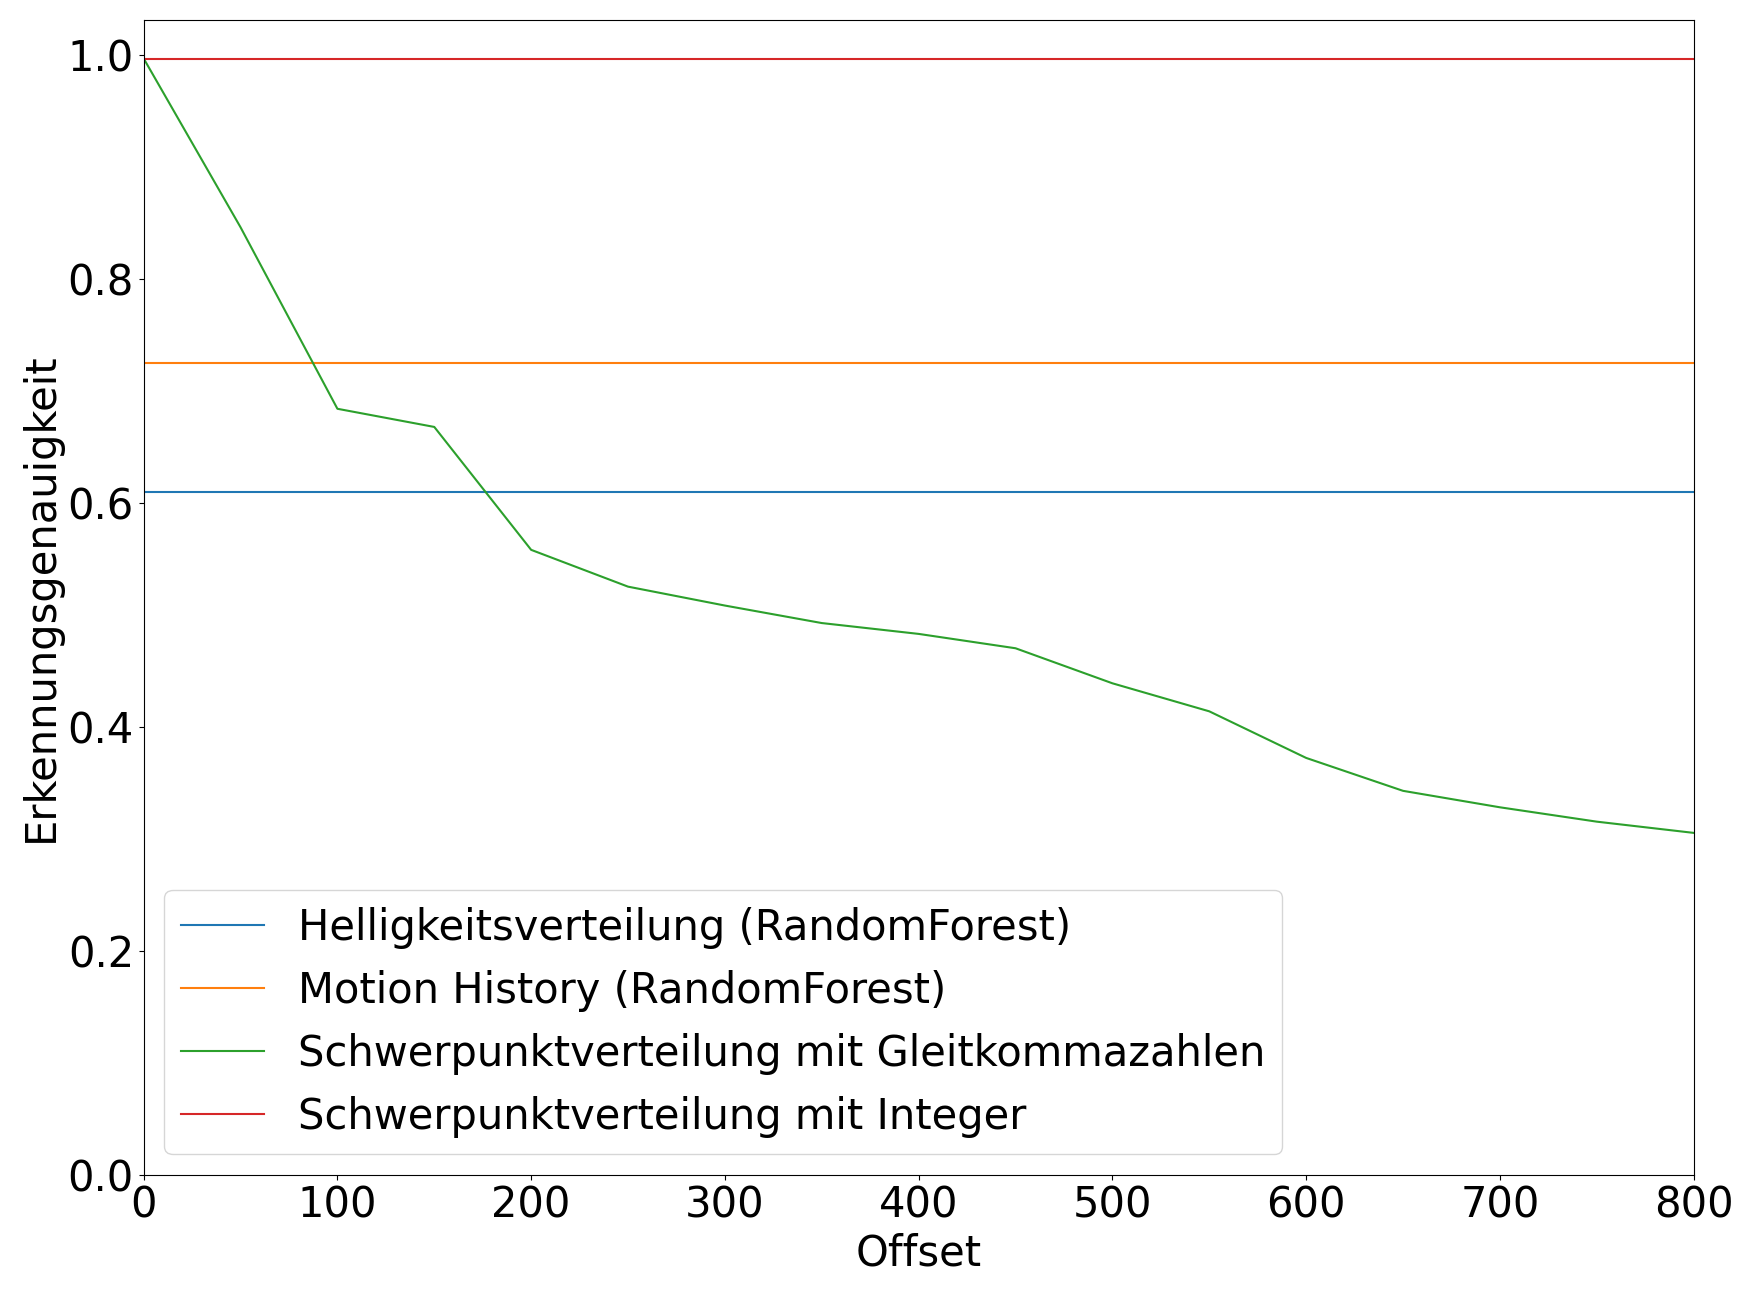
\includegraphics[width=\linewidth]{images/brightness_offset.png}
    \caption{Robustheit gegenüber einen ansteigenden Offset von der besten Konfiguration jedes Ansatzes.}
    \label{fig:brightness_offset}
\end{figure}
In Sektion \ref{sec:DymelData} wurde die Testmenge für die Lichtverhältnisse vorgestellt. Diese Testmenge modifiziert einen bestehenden Datensatz aus der Gestentestmenge von Dymel indem Offset hinzugefügt wird
oder die Helligkeiten skaliert werden. Bei dem Offset verändert sich der Kontrast nicht, aber die Gesamthelligkeit steigt. Bei der Skalierung steigt die Gesamthelligkeit und der Kontrast wird stärker. Mit
dieser Testmenge sollen die Invarianzen der einzelnen Ansätze bewertet werden.
\newline
\newline
Abbildung \ref{fig:brightness_offset} zeigt, dass die Helligkeitsverteilung, Motion History und die Schwerpunktverteilung
mit Integer invariant gegenüber einen offset sind, wohingegen die Schwerpunktverteilung mit Gleitkommazahlen starke Defiziete aufweist. Für die Helligkeitsverteilung und Motion History wurden die
Konfigurationen gewählt, die insgesamt am besten waren, da die Testmenge für Lichtverhältnisse auf der Gestentestmenge von Dymel basiert.
\begin{figure}[h!]
    \centering
    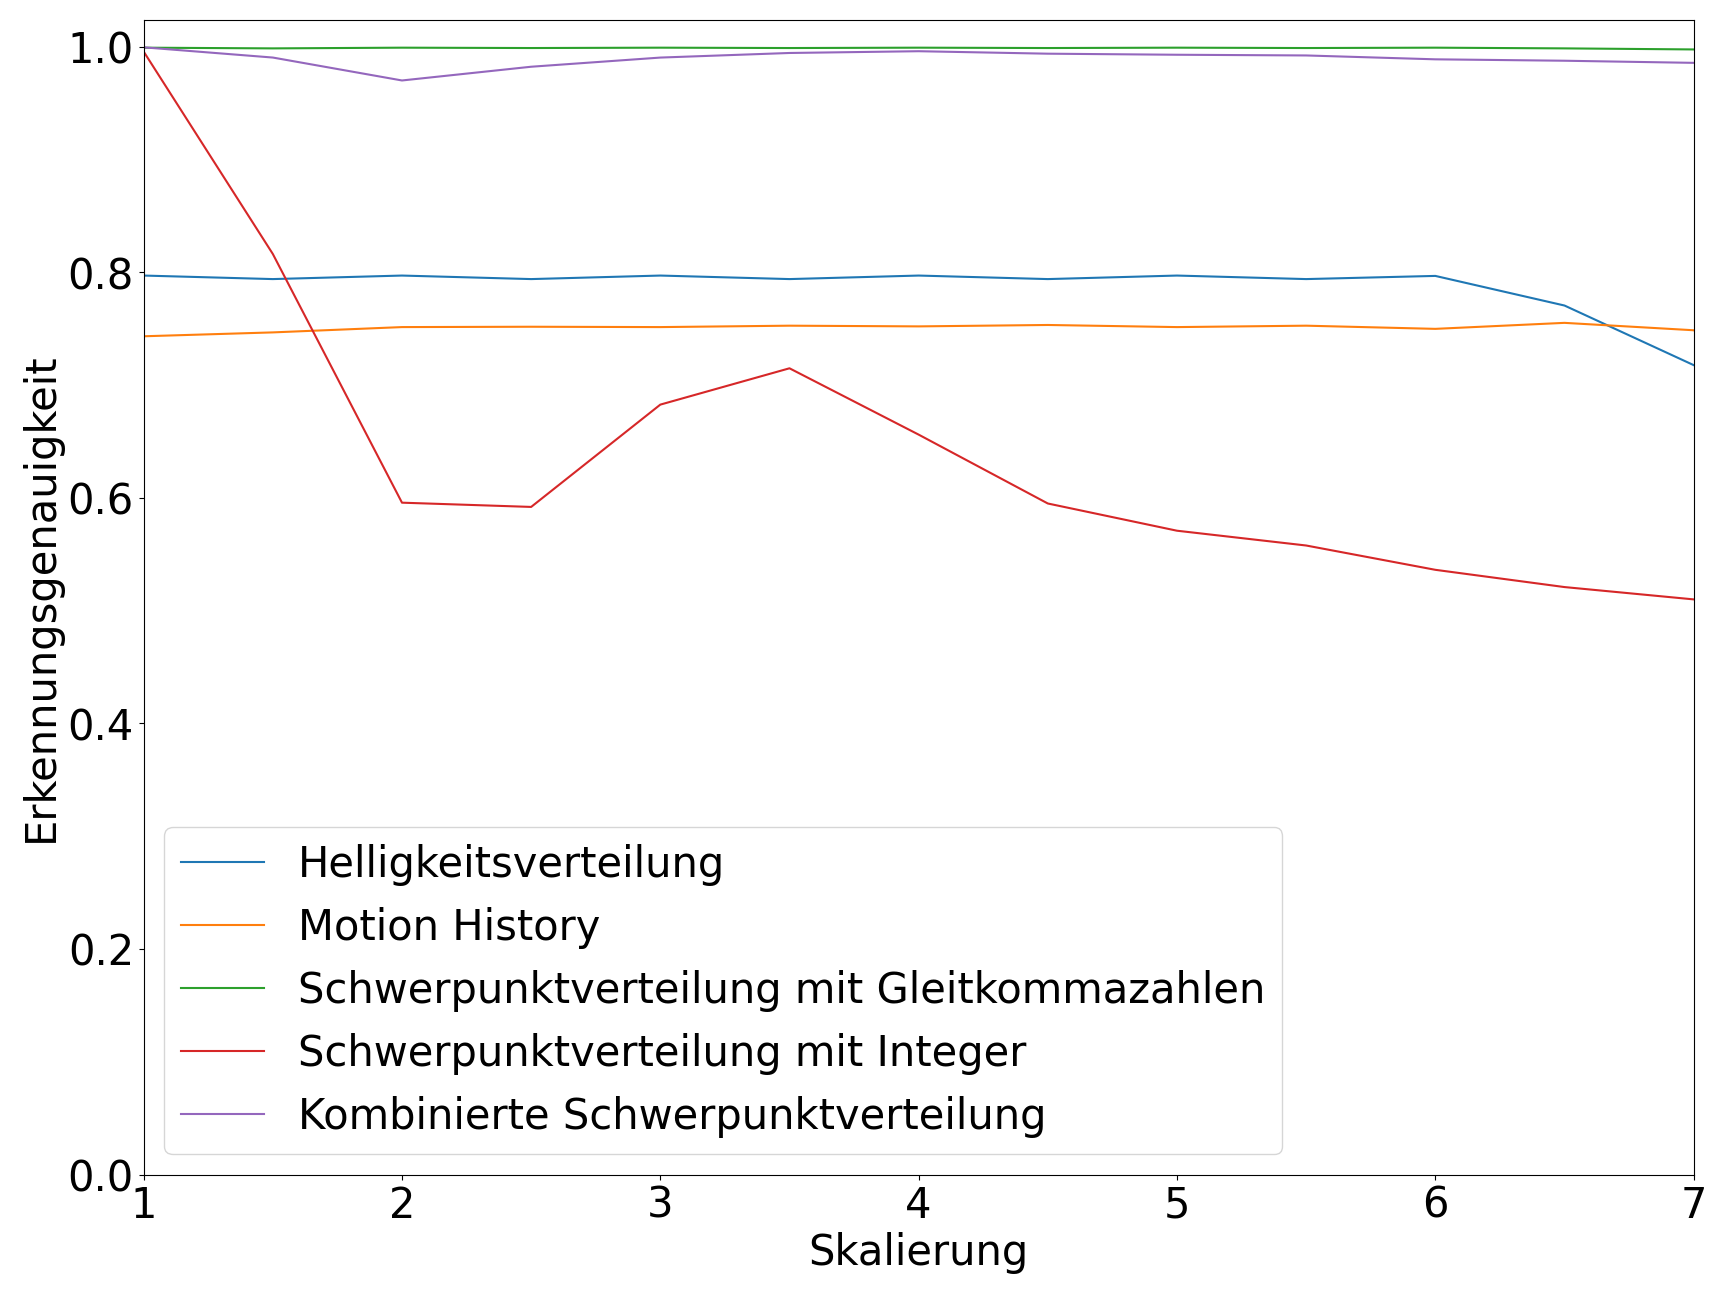
\includegraphics[width=\linewidth]{images/brightness_scaling.png}
    \caption{Robustheit gegenüber einer ansteigenden Skalierung von der besten Konfiguration jedes Ansatzes.}
    \label{fig:brightness_scaling}
\end{figure}
\newline
\newline
Abbildung \ref{fig:brightness_scaling} zeigt, dass die Schwerpunktverteilung mit Gleitkommazahlen invariant gegenüber Skalierung ist. Die Helligkeitsverteilung und Motion History weisen weitesgehend
keine Defiziete auf. Die Helligkeitsverteilung ist sogar zwischen der Skalierungstufe 6 und 7,5 besser. Die Schwerpunktverteilung mit Integer ist nicht invariant. Insgesamt verhalten sich alle Ansätze
wie erwartet. Die Skalierung \textit{0} bedeutet \glqq Keine Skalierung\grqq.
